\section{Temel Optimizasyon Kavramları}
Optimizasyon problemlerinin matematiksel olarak formüle edilmesi ve çözülmesi için gerekli olan temel kavramlar, bu bölümde detaylı olarak incelenecektir. Bu kavramlar, daha karmaşık optimizasyon problemlerinin anlaşılması için temel oluşturur.

\subsection{Amaç Fonksiyonu ve Kısıt Fonksiyonları}

Optimizasyon problemlerinin matematiksel modellemesinde iki temel bileşen vardır: amaç fonksiyonu ve kısıt fonksiyonları.

\subsubsection{Amaç Fonksiyonu}
Amaç fonksiyonu, optimize edilmek istenen performans kriterini matematiksel olarak ifade eder. Bu fonksiyon:
\begin{itemize}
    \item Minimize edilebilir (örn. maliyet, ağırlık, enerji tüketimi)
    \item Maksimize edilebilir (örn. verim, dayanım, rijitlik)
\end{itemize}

\begin{figure}[H]
    \centering
    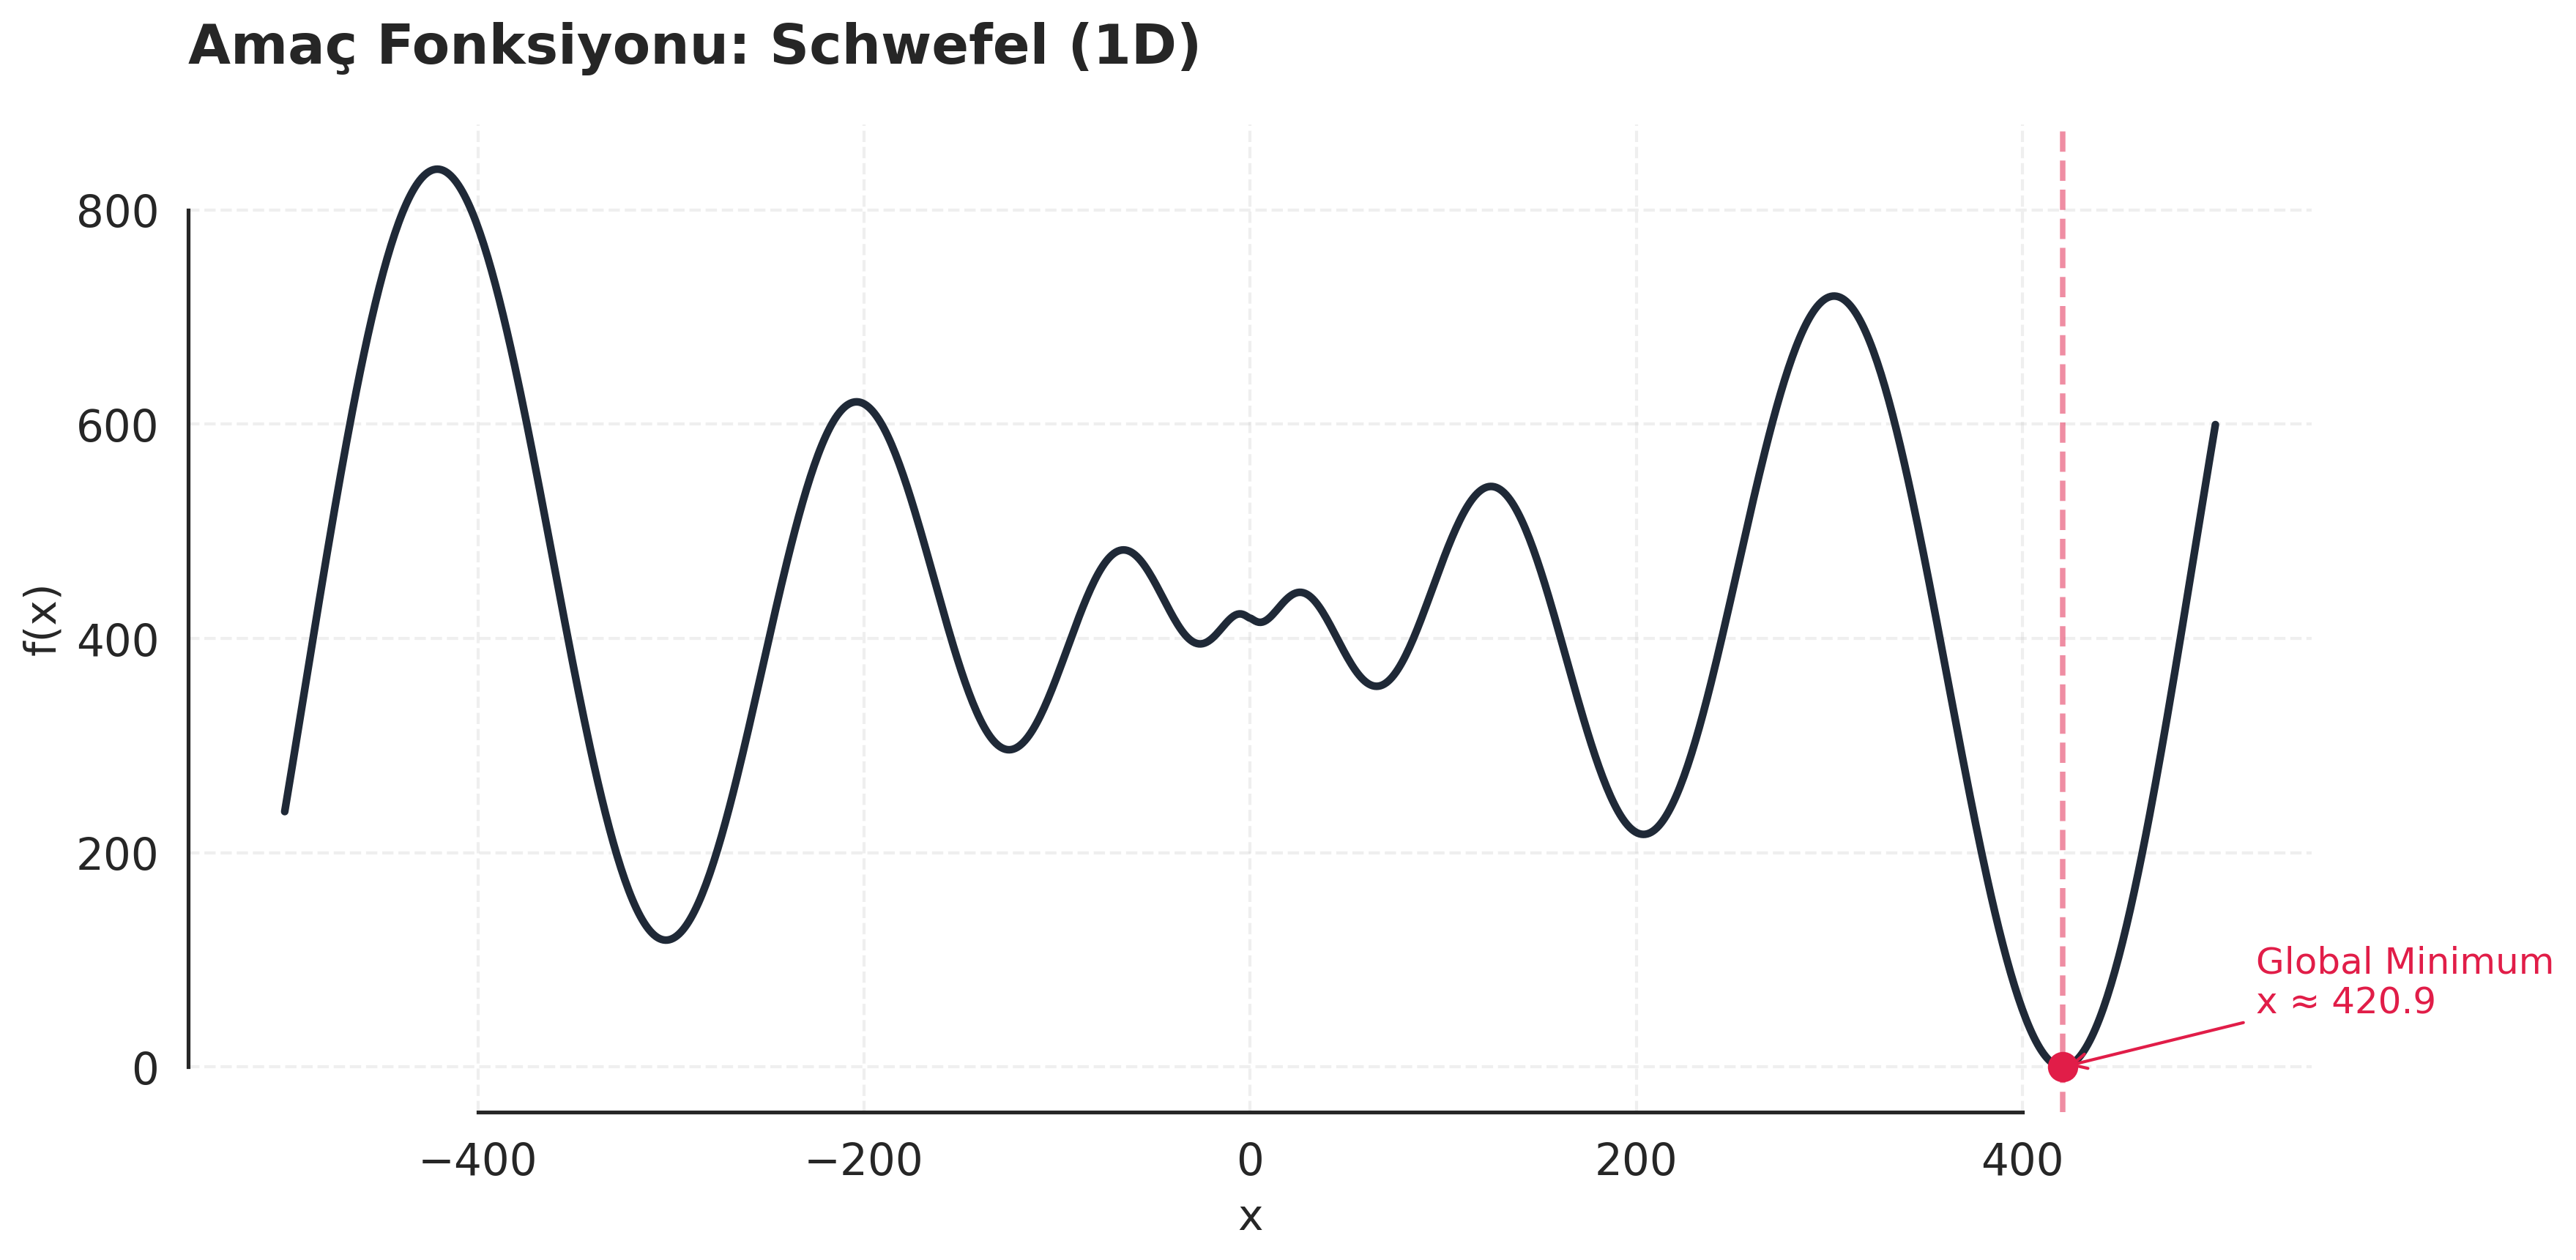
\includegraphics[width=1\textwidth]{weeks_new/imgs/objective_function.png}
    \caption{Amaç Fonksiyonu}
    \label{fig:multi_mod}
\end{figure}

\sidenote{Her maksimizasyon problemi, amaç fonksiyonunun negatifi alınarak bir minimizasyon problemine dönüştürülebilir: \[ \max f(x) = -\min(-f(x)) \]}

\subsubsection{Kısıt Fonksiyonları}
Kısıt fonksiyonları, tasarımın sağlaması gereken şartları matematiksel olarak ifade eder:
\begin{itemize}
    \item Eşitlik kısıtları: $h_j(x) = 0$
    \item Eşitsizlik kısıtları: $g_i(x) \leq 0$
    \item Sınır kısıtları: $x_L \leq x \leq x_U$ \sidenote{İstisnai durumlar haricinde yapısal optimizasyon problemleri genellikle eşitsizlik kısıtlarıyla ifade edilir. Probleme bağlı olarak sınır kısıtları da kullanılabilir. Ancak hiperstatik bir yapının optimizasyona konu olması halinde bu kısıtlayıcı, global optimumun ıskalanmasına da sebep olabilir.
    
    Aslında yapısal optimizasyon problemlerini optimizasyon açısından incelenmeye değer kılan noktalardan birisi de bu hiperstatiklik durumunun birçok yapısal optimizasyon probleminin öngörülmezliğini önemli ölçüde artırmasıdır.}
\end{itemize}


\textbf{Eşitlik kısıtları: $h_j(x) = 0$}
Eşitlik kısıtları, tasarım değişkenlerinin tam olarak belirli bir değer alması gereken durumları ifade eder. Bu tür kısıtlar, optimizasyon problemi içinde bazı parametrelerin kesin olarak sağlanması gereken şartları matematiksel olarak tanımlar. Örneğin, bir yapının toplam ağırlığının belirli bir değere eşit olması veya bir kimyasal reaksiyonda kütle dengesinin sağlanması gibi durumlar eşitlik kısıtlarıyla ifade edilebilir. Eşitlik kısıtları genellikle optimizasyon uzayını daha dar bir alanda tutarak, mümkün çözümlerin sayısını önemli ölçüde azaltır.


\begin{figure}[H]
    \centering
    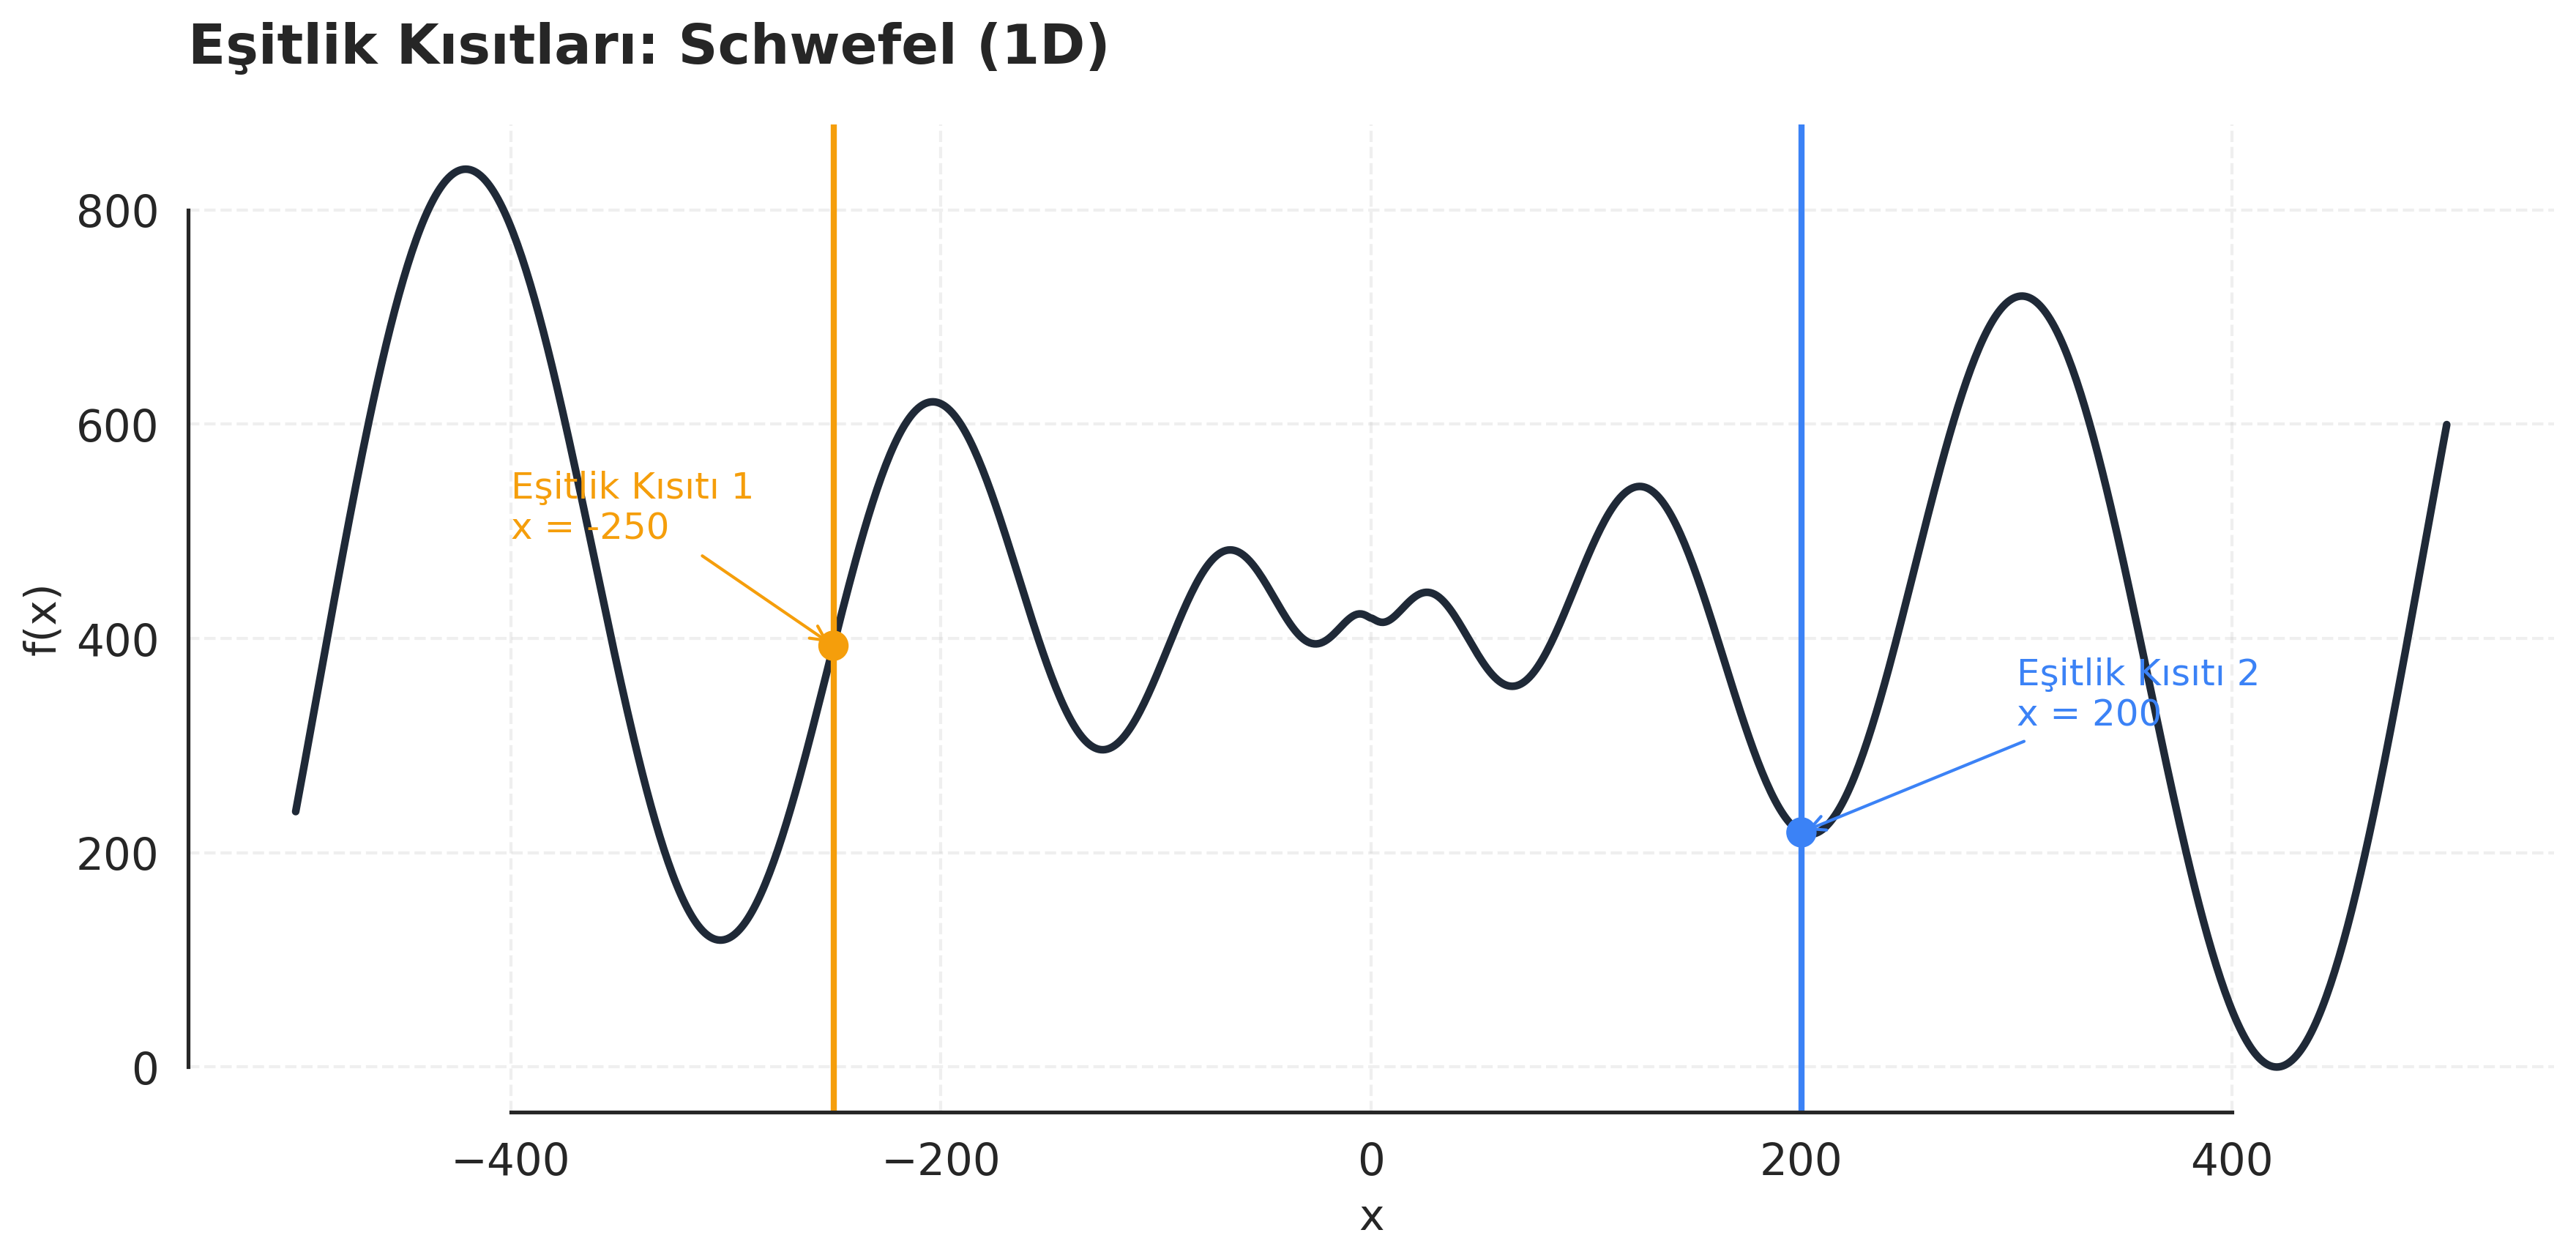
\includegraphics[width=1\textwidth]{weeks_new/imgs/equality_constraints.png}
    \caption{Eşitlik kısıtları}
    \label{fig:}
\end{figure}

\textbf{Eşitsizlik kısıtları: $g_i(x) \leq 0$}
Eşitsizlik kısıtları, tasarım değişkenlerinin belirli bir sınırı aşmaması gereken durumları ifade eder. Bu tür kısıtlar, bir yapının dayanabileceği maksimum gerilme değeri, bir sistemin maksimum enerji tüketimi veya bir malzemenin minimum güvenlik faktörü gibi sınırlamaları tanımlamak için kullanılır. Eşitsizlik kısıtları, tasarımın fiziksel olarak gerçeklenebilir ve güvenli olmasını sağlamak için kritik öneme sahiptir. Ayrıca eşitsizlik kısıtları, uygulanabilir çözüm alanını belirleyerek, optimizasyon algoritmasının yalnızca geçerli tasarım alanında arama yapmasını sağlar.

\begin{figure}[H]
    \centering
    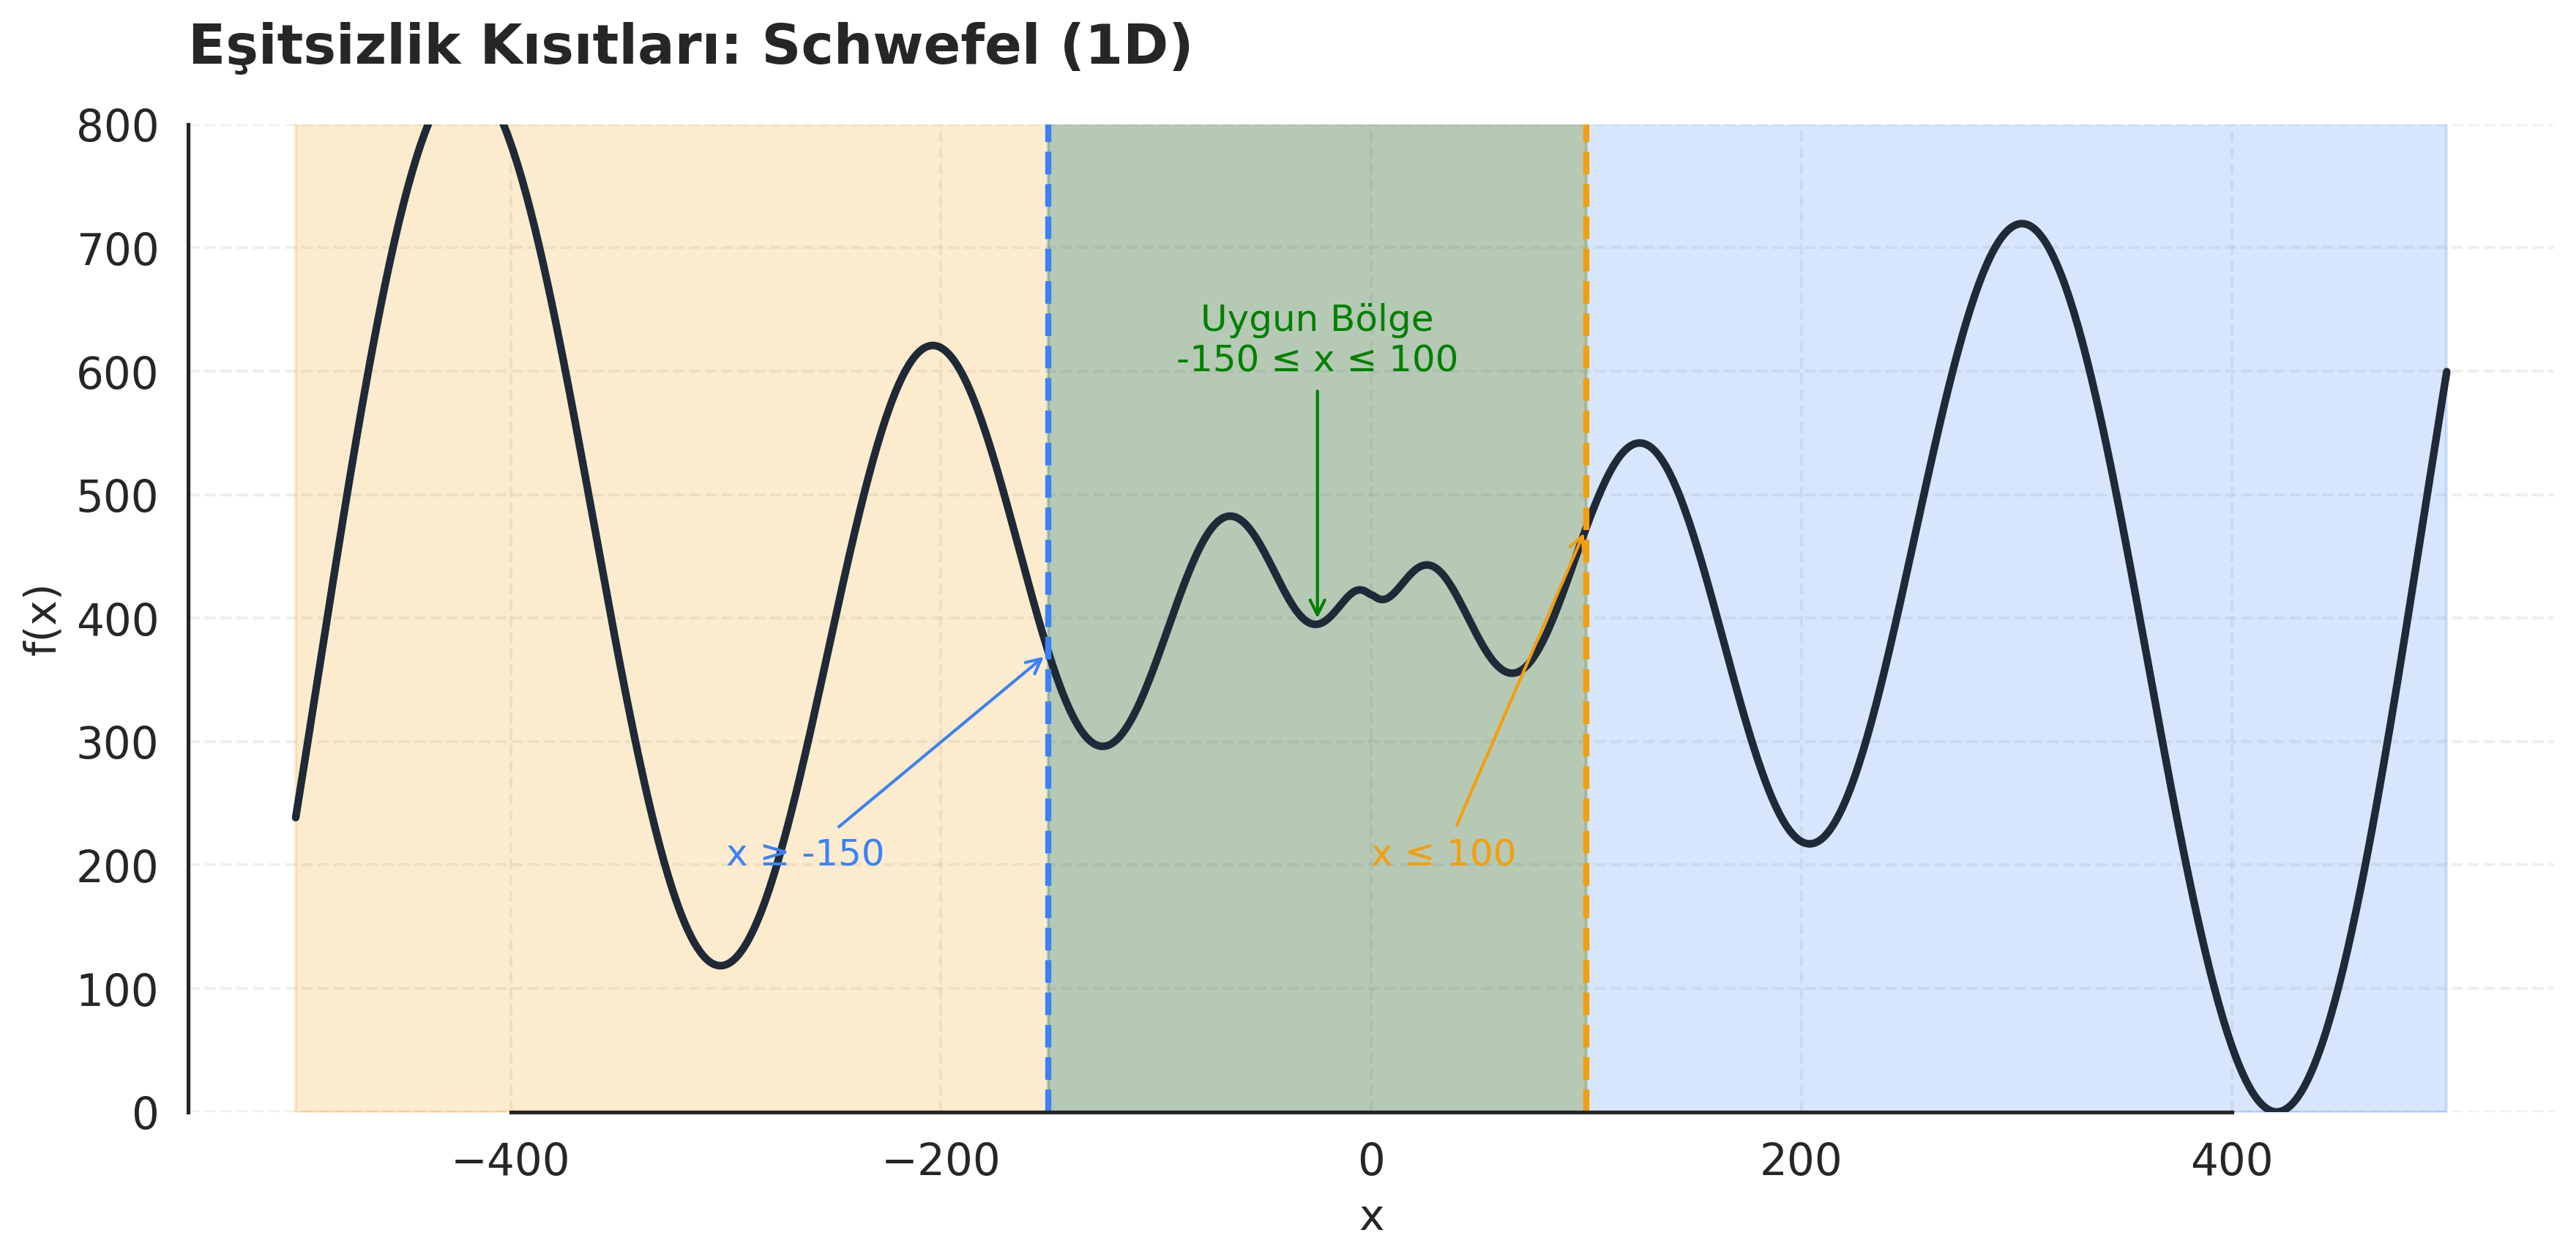
\includegraphics[width=1\textwidth]{weeks_new/imgs/inequality_constraints.png}
    \caption{Eşitsizlik kısıtları}
    \label{fig:}
\end{figure}


\textbf{Sınır kısıtları: $x_L \leq x \leq x_U$}
Sınır kısıtları, her bir tasarım değişkeninin alabileceği minimum ve maksimum değerleri belirleyen kısıtlardır. Bu kısıtlar, tasarım değişkenlerinin fiziksel sınırlarını, üretilebilirlik koşullarını veya standartlarca belirlenmiş aralıkları yansıtır. Örneğin, bir kirişin kalınlığının üretim kısıtları nedeniyle belirli bir değerden küçük olamayacağı veya kurulum gereksinimleri nedeniyle belirli bir maksimum değeri aşamayacağı durumlar sınır kısıtlarıyla ifade edilir. Sınır kısıtları, optimizasyon algoritmasının arama uzayını daraltarak, hesaplama verimliliğini artırır ve fiziksel olarak anlamsız çözümlerin elenmesini sağlar.

\begin{figure}[H]
    \centering
    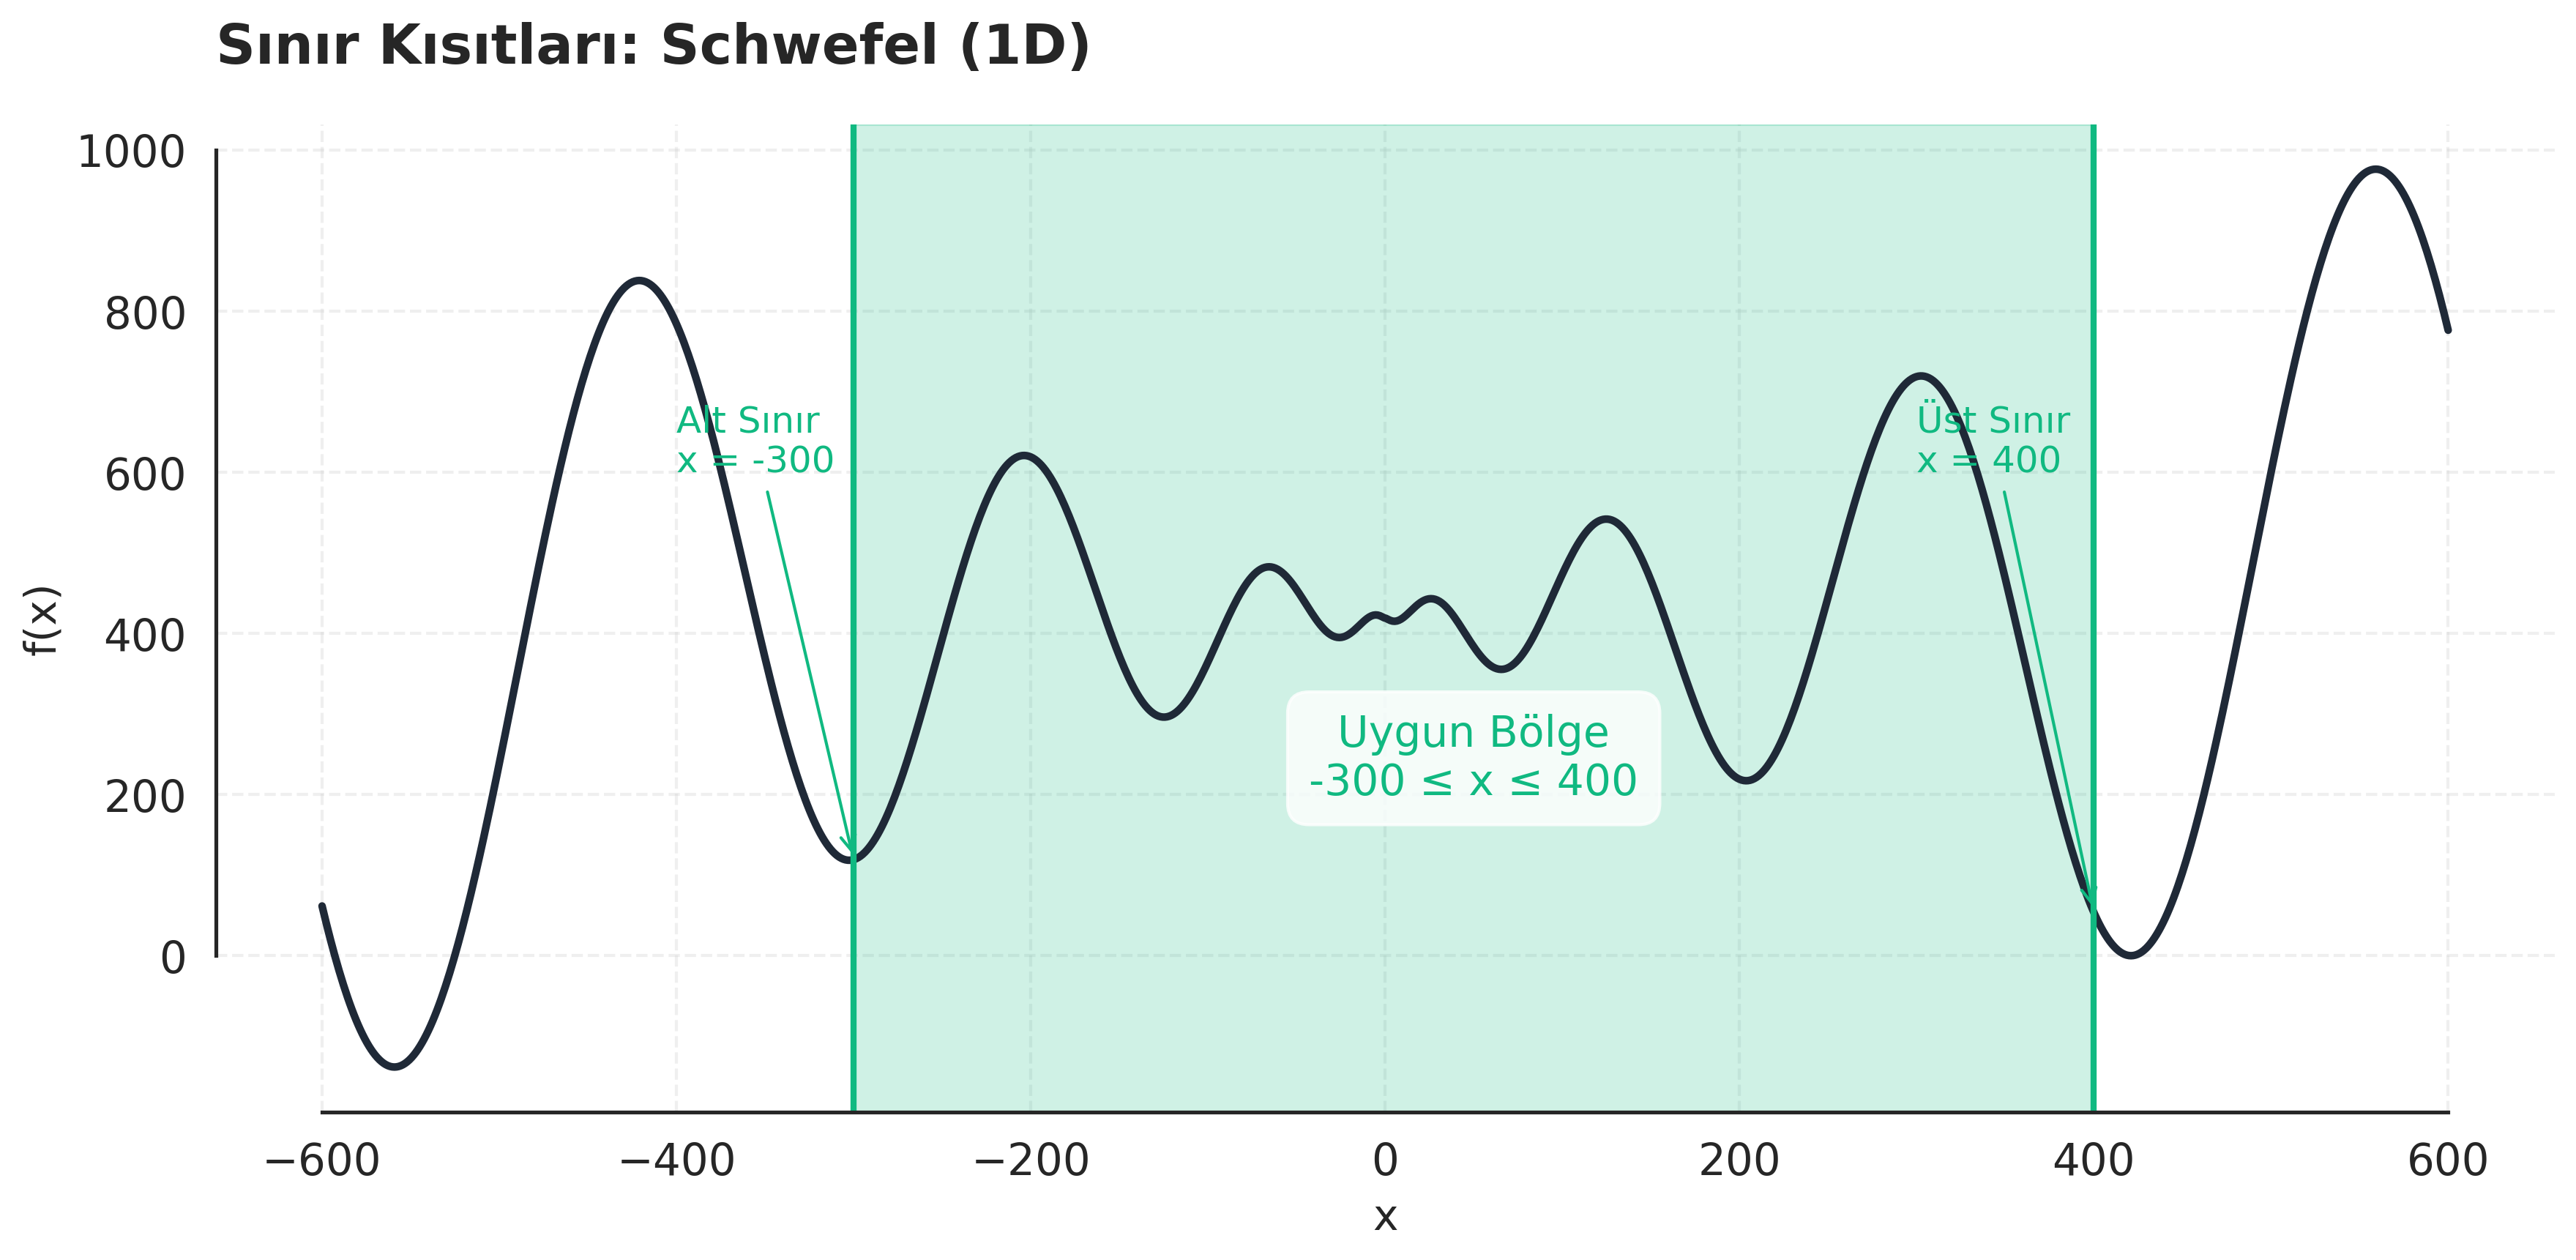
\includegraphics[width=1\textwidth]{weeks_new/imgs/boundary_constraints.png}
    \caption{Sınır Kısıtları}
    \label{fig:}
\end{figure}

\begin{marginfigure}
\centering
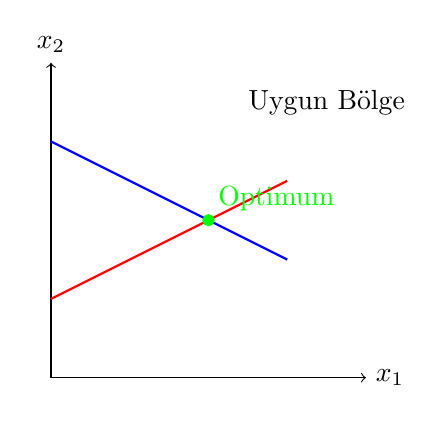
\begin{tikzpicture}
\draw[->] (0,0) -- (4,0) node[right] {$x_1$};
\draw[->] (0,0) -- (0,4) node[above] {$x_2$};
\draw[blue,thick] plot[smooth] coordinates {(0,3) (1,2.5) (2,2) (3,1.5)};
\draw[red,thick] plot[smooth] coordinates {(0,1) (1,1.5) (2,2) (3,2.5)};
\filldraw[green] (2,2) circle (2pt) node[above right] {Optimum};
\node at (3.5,3.5) {Uygun Bölge};
\end{tikzpicture}
\caption{İki kısıtın kesişimi ile oluşan uygun çözüm bölgesi}
\label{fig:feasible_region}
\end{marginfigure}

\subsection{Karar Değişkenleri ve Çözüm Uzayı}

\subsubsection{Karar Değişkenleri}
Karar değişkenleri, optimizasyon sürecinde değerleri belirlenmesi gereken parametrelerdir:
\begin{itemize}
    \item Sürekli (Continuous) değişkenler (örn. boyutlar, kalınlıklar)
    \item Tamsayı (Discrete) değişkenler (örn. eleman sayısı)
    \item İkili (Binary) değişkenler (0-1 kararları)
\end{itemize}

\begin{tcolorbox}[title=Yapısal Tasarımda Karar Değişkenleri]
Bir çelik çerçeve optimizasyonunda:
\begin{itemize}
    \item \textbf{Sürekli:} Kesit boyutları
    \item \textbf{Tamsayı:} Kat sayısı
    \item \textbf{İkili:} Elemanların varlığı/yokluğu
\end{itemize}
\end{tcolorbox}

\subsubsection{Çözüm Uzayı}
Çözüm uzayı, tüm olası karar değişkeni kombinasyonlarının oluşturduğu uzaydır\sidenote{Çözüm uzayının boyutu, karar değişkenlerinin sayısı ile belirlenir. Yüksek boyutlu problemlerde "lanet boyut" (curse of dimensionality) problemi ortaya çıkar.}:
\begin{itemize}
    \item \textbf{Uygun Çözüm Bölgesi:} Tüm kısıtları sağlayan noktalar kümesi
    \item \textbf{Uygun Olmayan Bölge:} En az bir kısıtı ihlal eden noktalar
\end{itemize}


\subsection{Global ve Yerel (Lokal) Minimum/Maksimum Kavramları}

\subsubsection{Yerel Optimum}
Bir nokta, belirli bir komşuluk içinde en iyi değere sahipse yerel optimumdur:
\begin{equation}
x^* \text{ yerel minimum } \Leftrightarrow f(x^*) \leq f(x), \forall x \in N(x^*)
\end{equation}

\subsubsection{Global Optimum}
Tüm çözüm uzayında en iyi değere sahip nokta global optimumdur:
\begin{equation}
x^* \text{ global minimum } \Leftrightarrow f(x^*) \leq f(x), \forall x \in S
\end{equation}

\begin{figure}
\centering
\begin{tikzpicture}
\draw[->] (0,0) -- (7,0) node[right] {$x$};
\draw[->] (0,-1) -- (0,4) node[above] {$f(x)$};
\draw[scale=1,domain=0:7,smooth,variable=\x,blue] plot ({\x},{1 + sin(3*\x r)+sin(\x r)+sin(0.5*\x r)});
\filldraw[gray] (1.526,1.699) circle (2pt) node[below] {Lokal};
\filldraw[gray] (3.774,0.412) circle (2pt) node[below] {Lokal};
\filldraw[black] (5.719,-0.249) circle (2pt) node[below] {Global};
\end{tikzpicture}
\caption{Bir fonksiyonun yerel ve global minimum noktaları}
\label{fig:local_global}
\end{figure}

\subsection{Fiziksel ve Matematiksel Modelleme}

\subsubsection{Fiziksel Modelleme}
Gerçek dünya probleminin fiziksel prensiplere dayalı olarak modellenmesi\sidenote{İyi bir matematiksel model, fiziksel gerçekliği yeterli doğrulukta yansıtmalı, ancak gereksiz karmaşıklıktan kaçınmalıdır. Bu esasen optimizasyonun başlıca konusu olmasa da yapısal optimizasyon açısından oldukça önemli bir konudur.}:
\begin{itemize}
    \item Kuvvet dengesi
    \item Enerji korunumu
    \item Malzeme davranışı
    \item Geometrik ilişkiler
\end{itemize}

\subsubsection{Matematiksel Modelleme}
Fiziksel modelin matematiksel formülasyona dönüştürülmesi:
\begin{itemize}
    \item Diferansiyel denklemler
    \item Cebirsel denklemler
    \item Matris formülasyonları
    \item Sonlu eleman modelleri
\end{itemize}

\subsection{Diferansiyellenebilirlik ve Süreklilik}

\subsubsection{Süreklilik}
Fonksiyonun sürekli olması, küçük girdi değişimlerinin çıktıda ani sıçramalara neden olmaması demektir. Matematiksel olarak:
\begin{equation}
\lim_{x \to x_0} f(x) = f(x_0)
\end{equation}

\begin{tcolorbox}[title=Süreklilik ve Optimizasyon İlişkisi]
Süreklilik, optimizasyon problemlerinde önemli bir özelliktir çünkü:
\begin{itemize}
    \item Sürekli fonksiyonlar için kapalı ve sınırlı bir aralıkta mutlaka bir minimum ve maksimum değer vardır (Weierstrass teoremi).
    \item Sürekli olmayan fonksiyonların optimizasyonu daha zordur çünkü ani sıçramalar, algoritmaların doğru yönde ilerlemesini engelleyebilir.
    \item Gerçek mühendislik problemlerinde çoğu fiziksel davranış, sürekli fonksiyonlarla modellenir (örneğin, bir kirişin yük altında deformasyonu).
\end{itemize}
\end{tcolorbox}

\subsubsection{Diferansiyellenebilirlik}
Fonksiyonun türevinin var olması, fonksiyonun davranışının her noktada bir teğet doğru ile yaklaşık olarak ifade edilebilmesi anlamına gelir. Matematiksel olarak:
\begin{equation}
f'(x_0) = \lim_{h \to 0} \frac{f(x_0 + h) - f(x_0)}{h}
\end{equation}

\begin{tcolorbox}[title=Diferansiyellenebilirlik ve Optimizasyon Arasındaki İlişki]
Diferansiyellenebilirlik, optimizasyon sürecinde kritik bir role sahiptir:
\begin{itemize}
    \item \textbf{Gradyan Bilgisi:} Türev, fonksiyonun en hızlı artış/azalış yönünü verir, böylece optimizasyon algoritmaları nereye gideceklerini bilir.
    \item \textbf{Kritik Noktalar:} Fonksiyonun türevinin sıfır olduğu noktalar (kritik noktalar), potansiyel optimum noktalardır.
    \item \textbf{İkinci Türev:} İkinci türev, kritik noktanın minimum, maksimum veya eğer noktası olduğunu belirlemede yardımcı olur.
\end{itemize}
\end{tcolorbox}

\begin{marginfigure}
    \centering
    \begin{tikzpicture}
    \draw[->] (0,0) -- (6,0) node[right] {$x$};
    \draw[->] (0,0) -- (0,4) node[above] {$f(x)$};
    
    % Fonksiyon
    \draw[blue, thick, domain=0:6, smooth, variable=\x] plot ({\x}, {0.1*\x*\x*\x - 0.9*\x*\x + 2*\x + 0.5});
    
    \end{tikzpicture}
    \caption{Diferansiyellenebilir Fonksiyon ve Gradyan}
    \label{fig:differentiability}
\end{marginfigure}

\begin{marginfigure}
    \centering
    \begin{tikzpicture}
    \draw[->] (0,0) -- (6,0) node[right] {$x$};
    \draw[->] (0,0) -- (0,4) node[above] {$f(x)$};
    
    % Diferansiyellenemeyen fonksiyon (mutlak değer)
    \draw[blue, thick, domain=0:3, smooth, variable=\x] plot ({\x}, {3-\x});
    \draw[blue, thick, domain=3:6, smooth, variable=\x] plot ({\x}, {\x-3});
    
    % Kritik nokta (köşe)
    \filldraw[red] (3,0) circle (2pt) node[below right] {$f'(x)$ tanımsız};
    
    \end{tikzpicture}
    \caption{Diferansiyellenemeyen Fonksiyon (Mutlak Değer Fonksiyonu)}
    \label{fig:non_differentiable}
\end{marginfigure}

\begin{tcolorbox}[title=Gerçek Hayat Örneği: Tepeye Tırmanma]
Düşünün ki bir dağa tırmanıyorsunuz ve hedefiniz zirveye ulaşmak. Eğer sisli bir günde görüş alanınız çok kısıtlıysa, nasıl ilerlemelisiniz?

\begin{itemize}
    \item \textbf{Gradyan (Türev) Bilgisi:} Her adımda ayaklarınızla zeminin eğimini hissederek en dik yokuş yukarı yönünü (negatif gradyan) seçebilirsiniz.
    \item \textbf{Diferansiyellenemeyen Noktalar:} Eğer yolunuz üzerinde dik bir kayalık (türevin tanımlanamadığı nokta) varsa, doğrudan ilerleyemez, farklı bir yol bulmanız gerekir.
    \item \textbf{Yerel Tepe vs. Zirve:} Tırmanışınız sırasında küçük bir tepeye (yerel maksimum) ulaşabilirsiniz, ancak gerçek zirve (global maksimum) başka bir yerde olabilir.
\end{itemize}

Bu anoloji, gradyan tabanlı optimizasyon algoritmalarının çalışma prensibine çok benzerdir.
\end{tcolorbox}


\begin{tcolorbox}[title=Diferansiyellenebilirliğe Göre Optimizasyon Yöntemleri]
\begin{itemize}
    \item \textbf{Diferansiyellenebilir Fonksiyonlar için Gradyan Tabanlı Yöntemler:}
    \begin{itemize}
        \item \textbf{Gradyan İniş:} Fonksiyonun en hızlı düşüş yönünde ilerler.
        \item \textbf{Newton Yöntemi:} İkinci türev bilgisini kullanarak daha hızlı yakınsama sağlar.
        \item \textbf{Quasi-Newton:} İkinci türevi yaklaşık olarak hesaplar (BFGS, L-BFGS gibi).
    \end{itemize}
    
    \item \textbf{Diferansiyellenemeyen Fonksiyonlar için Gradyan-sız Yöntemler:}
    \begin{itemize}
        \item \textbf{Simpleks Arama:} Fonksiyon değerlerini karşılaştırarak en uygun yönü belirler (Nelder-Mead yöntemi).
        \item \textbf{Genetik Algoritmalar:} Evrimsel süreçleri taklit ederek çözüm uzayını araştırır.
        \item \textbf{Parçacık Sürü Optimizasyonu:} Grup davranışını taklit ederek çözüme yaklaşır.
    \end{itemize}
    
    \item \textbf{Karma Problemler için Hibrit Yaklaşımlar:}
    \begin{itemize}
        \item \textbf{Arama + İyileştirme:} Gradyan-sız bir yöntemle geniş bölgede arama, sonra bulduğu noktadan gradyan tabanlı yöntemle iyileştirme.
        \item \textbf{Alt-Gradyan Yöntemleri:} Diferansiyellenemeyen noktalarda bile ilerleme sağlayan genelleştirilmiş türev yaklaşımları.
    \end{itemize}
\end{itemize}
\end{tcolorbox}\sidenote{Yapısal optimizasyon problemleri genellikle diferansiyellenebilir değildir. Bu nedenle, global optimumu bulmak zorlaşır ve metasezgisel yöntemler tercih edilir.}



\subsection{Konveks ve Konveks Olmayan Optimizasyon}

\subsubsection{Konveks Fonksiyonlar}
Bir fonksiyonun konveks olması, fonksiyonun grafiğinin herhangi iki noktasını birleştiren doğru parçasının, bu iki nokta arasındaki fonksiyon grafiğinin üzerinde kalması demektir. Matematiksel olarak, $f: \mathbb{R}^n \rightarrow \mathbb{R}$ fonksiyonu için:
\begin{equation}
f(\lambda x + (1-\lambda)y) \leq \lambda f(x) + (1-\lambda) f(y), \quad \forall x,y \in \mathbb{R}^n, \forall \lambda \in [0,1]
\end{equation}

\begin{figure}[H]
    \centering
    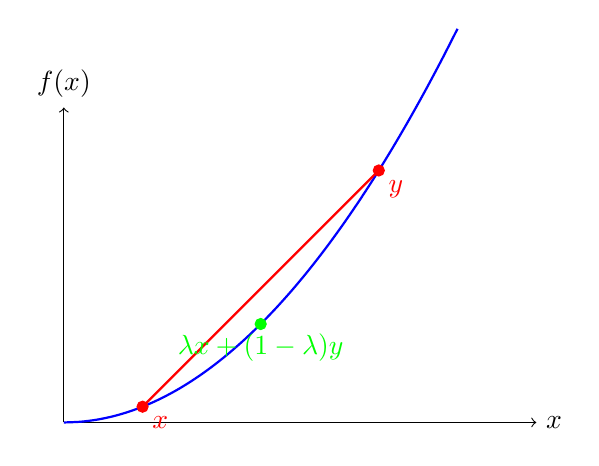
\begin{tikzpicture}
    \draw[->] (0,0) -- (6,0) node[right] {$x$};
    \draw[->] (0,0) -- (0,4) node[above] {$f(x)$};
    
    % Konveks fonksiyon
    \draw[blue, thick, domain=0:5, smooth, variable=\x] plot ({\x}, {0.2*\x*\x});
    
    % İki nokta
    \filldraw[red] (1,0.2) circle (2pt) node[below right] {$x$};
    \filldraw[red] (4,3.2) circle (2pt) node[below right] {$y$};
    
    % Doğru parça
    \draw[red, thick] (1,0.2) -- (4,3.2);
    
    % Orta nokta
    \filldraw[green] (2.5,1.25) circle (2pt) node[below] {$\lambda x + (1-\lambda)y$};
    
    \end{tikzpicture}
    \caption{Konveks Fonksiyon Örneği}
    \label{fig:convex_function}
\end{figure}

\subsubsection{Konveks Küme}
Konveks bir küme, küme içindeki herhangi iki noktayı birleştiren doğru parçasının tamamen küme içinde kalması anlamına gelir:
\begin{equation}
\lambda x + (1-\lambda)y \in S, \quad \forall x,y \in S, \forall \lambda \in [0,1]
\end{equation}

\begin{figure}[H]
    \centering
    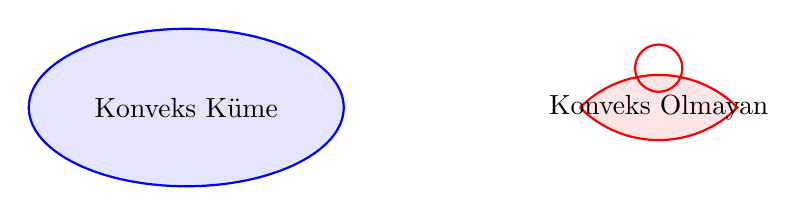
\begin{tikzpicture}
    % Konveks küme
    \draw[blue, thick, fill=blue!10] (0,0) ellipse (2 and 1);
    \node at (0,0) {Konveks Küme};
    
    % Konveks olmayan küme
    \draw[red, thick, fill=red!10] (5,0) to[out=45,in=135] (7,0) to[out=-135,in=-45] (5,0);
    \draw[red, thick] (6,0.5) circle (0.3);
    \node at (6,0) {Konveks Olmayan};
    \end{tikzpicture}
    \caption{Konveks ve Konveks Olmayan Küme Örnekleri}
    \label{fig:convex_nonconvex_sets}
\end{figure}

\subsubsection{Konveks Optimizasyon Avantajları}
Konveks optimizasyon, optimizasyon teorisinde özel bir öneme sahiptir\sidenote{Konveks optimizasyon problemleri için geliştirilmiş etkili algoritmalar ve matematiksel garantiler, bu tür problemlerin çözümünü daha güvenilir hale getirir. Günümüzde sıkça duyduğumuz derin öğrenme algoritmalarının içinde yer alan optimizasyon problemleri genellikle konveks optimizasyon problemleridir. Burada kullanılan optimizasyon algoritmaları genellikle gradyan iniş yöntemleridir. Çok efektif yöntemler olmalarının yanında genellikle yapısaal optimizasyon problemlerinde verimsiz kalırlar. }:

\begin{itemize}
    \item \textbf{Yerel Optimum = Global Optimum:} Konveks bir fonksiyonun yerel minimumu, aynı zamanda global minimumdur. Bu, optimizasyon sürecini önemli ölçüde basitleştirir.
    \item \textbf{Kararlı Çözüm:} Başlangıç noktasından bağımsız olarak, uygun gradyan tabanlı algoritmalar aynı optimum noktaya yakınsar.
    \item \textbf{Verimli Algoritmalar:} İç nokta yöntemleri, gradyan iniş yöntemi gibi algoritmalar konveks problemlerde polinom zamanda çözüme ulaşabilir.
\end{itemize}

\begin{tcolorbox}[title=Konveks Optimizasyon Örneği]
Karesel programlama problemi:
\begin{equation}
\begin{aligned}
\min_{x \in \mathbb{R}^n} & \quad \frac{1}{2}x^TQx + c^Tx \\
\text{s.t.} & \quad Ax \leq b
\end{aligned}
\end{equation}

Eğer $Q$ pozitif yarı-tanımlı bir matris ise, bu problem konvekstir ve verimli iç nokta yöntemleriyle çözülebilir.
\end{tcolorbox}

\subsubsection{Konveks Olmayan Optimizasyon Zorlukları}
Konveks olmayan optimizasyon problemleri, yapısal optimizasyonda sıklıkla karşılaşılan zorluklardır\sidenote{Yapısal optimizasyon problemlerinin çoğu, birden fazla yerel optimum içerebilen konveks olmayan problemlerdir. Bu da global optimumu bulma konusunda güçlükler yaratır.}:

\begin{itemize}
    \item \textbf{Çoklu Yerel Optimumlar:} Fonksiyon birden fazla yerel minimum içerebilir, bu nedenle global optimumu bulmak zorlaşır.
    \item \textbf{Başlangıç Noktası Bağımlılığı:} Gradyan tabanlı algoritmalar, başlangıç noktasına bağlı olarak farklı yerel optimumlara yakınsayabilir.
    \item \textbf{Hesaplama Maliyeti:} Global optimumu bulma garantisi için genellikle daha kapsamlı arama yöntemleri gereklidir, bu da hesaplama maliyetini artırır.
\end{itemize}


\begin{tcolorbox}[title=Konveks Olmayan Problemlere Yaklaşımlar]
\begin{itemize}
    \item \textbf{Çoklu Başlangıç Noktası:} Farklı başlangıç noktalarından birden fazla yerel optimizasyon çalıştırılarak en iyi sonuç seçilir.
    \item \textbf{Metasezgisel Algoritamalar:} Genetik algoritmalar, parçacık sürü optimizasyonu gibi yöntemler, geniş çözüm uzayını araştırarak global optimuma yaklaşmaya çalışır.
    \item \textbf{Konveks Yaklaşımlar:} Problemi konveks alt-problemlere ayrıştırarak veya konveks yaklaşımlar kullanarak çözüm aranabilir (Sequential Convex Programming gibi).
\end{itemize}
\end{tcolorbox}


\subsection{Kısıtsız ve Kısıtlı Optimizasyon}

\subsubsection{Kısıtsız Optimizasyon}
Kısıtsız optimizasyon, adından da anlaşılacağı gibi herhangi bir kısıt içermeyen, sadece amaç fonksiyonunun minimize veya maksimize edilmesi gereken problemleri ifade eder. Matematiksel olarak:
\begin{equation}
\min_{x \in \mathbb{R}^n} f(x)
\end{equation}

\sidenote{Kısıtsız optimizasyon, her ne kadar teorik olarak "kısıtsız" olarak adlandırılsa da, pratikte çoğu mühendislik problemi bir şekilde fiziksel veya matematiksel kısıtlar içerir. Buradaki "kısıtsız" terimi, problemin formülasyonunda açık kısıtlar olmadığı anlamına gelir.}

Kısıtsız optimizasyon problemlerini çözmek için kullanılan başlıca yöntemler \sidenote{Bu beş yöntemin çalışma biçimini test eden python kodu, bağlantı üzerinden test edilebilir. 

\qrcode[height=1in]{https://github.com/btayfur/structural-optimization/blob/main/Code/Examples/Exmp2/}}:

\begin{itemize}
    \item \textbf{Gradyan İniş Yöntemi:} Fonksiyonun en hızlı düşüş yönünde (negatif gradyan yönünde) adım adım ilerleyerek minimuma ulaşmayı hedefler. Bu yöntem, özellikle derin öğrenme ve makine öğrenmesi uygulamalarında yaygın olarak kullanılır.
    
    \item \textbf{Newton Yöntemi:} Fonksiyonun ikinci türev (Hessian) bilgisini de kullanarak, hem yön hem de adım büyüklüğü konusunda daha akıllı kararlar verir. Kuadratik yakınsama özelliği sayesinde, doğru koşullar altında gradyan inişinden daha hızlı yakınsar.
    
    \item \textbf{Quasi-Newton Yöntemleri:} Newton yönteminin hesaplama maliyetini düşürmek için Hessian matrisini doğrudan hesaplamak yerine, yaklaşık olarak tahmin eden yöntemlerdir. BFGS ve L-BFGS en popüler Quasi-Newton algoritmaları arasındadır.
    
    \item \textbf{Eş Gradyan Yöntemi (Conjugate Gradient):} Özellikle büyük ölçekli problemlerde etkili olan ve ardışık arama yönlerinin birbirine "eş" (conjugate) olmasını sağlayan bir yöntemdir.
    
    \item \textbf{Trust Region Yöntemleri:} Her iterasyonda, fonksiyonun yerel olarak iyi modellenebileceği bir "güven bölgesi" belirleyerek bu bölge içinde optimum arayan yöntemlerdir.
\end{itemize}



\begin{tcolorbox}[title=Dağa Tırmanma Analojisi]
Kısıtsız optimizasyon yöntemlerini anlamak için bir dağ tırmanışı analojisi düşünelim (maksimizasyon problemi için):

\begin{itemize}
    \item \textbf{Gradyan Tırmanışı:} Her adımda en dik yokuş yukarı yönde ilerlersiniz. Kolay uygulanır ancak dar vadilerde zigzaglar çizerek yavaş ilerleyebilir.
    
    \item \textbf{Newton Yöntemi:} Sadece zeminin eğimine (gradyan) değil, aynı zamanda arazinin şeklini (Hessian) de bakarsınız. Bu, düz alanlarda büyük adımlar atmanızı, dik yamaçlarda küçük ve dikkatli adımlar atmanızı sağlar.
    
    \item \textbf{Quasi-Newton:} Arazinin şeklini tam ölçmek yerine, önceki adımlarınızdan tahmin edersiniz. Bu, Newton kadar etkili olmasa da çok daha az çaba gerektirir.
\end{itemize}
\end{tcolorbox}

\subsubsection{Kısıtlı Optimizasyon}
Kısıtlı optimizasyon, gerçek dünya problemlerinin modellenmesinde çok daha yaygındır ve amaç fonksiyonunun yanı sıra bir dizi kısıt içerir. Bu kısıtlar, çözümün sağlaması gereken şartları temsil eder. Matematiksel formülasyonu:
\begin{equation}
\begin{aligned}
\min_{x \in \mathbb{R}^n} & \quad f(x) \\
\text{s.t.} & \quad g_i(x) \leq 0, \quad i = 1,\ldots,m \\
& \quad h_j(x) = 0, \quad j = 1,\ldots,p
\end{aligned}
\end{equation}

Burada $g_i(x) \leq 0$ eşitsizlik kısıtlarını, $h_j(x) = 0$ ise eşitlik kısıtlarını temsil eder.

\sidenote{Yapısal optimizasyon problemleri neredeyse her zaman kısıtlı problemlerdir. Bir köprünün ağırlığını minimize etmek istediğinizde, köprünün belirli yükleri taşıyabilmesi, belirli bir güvenlik faktörüne sahip olması ve inşa edilebilir olması gibi çeşitli kısıtlar vardır. Bu kısıtlar olmadan yapılan bir optimizasyon, pratikte uygulama alanı bulamaz.}

Kısıtlı optimizasyon problemlerini çözmek için kullanılan başlıca yöntemler:

\begin{itemize}
    \item \textbf{Lagrange Çarpanları Yöntemi:} Eşitlik kısıtlı problemler için Lagrange çarpanları adı verilen ek değişkenler tanımlayarak, kısıtlı problemi genişletilmiş bir kısıtsız probleme dönüştürür. Bu yöntem, kısıtların tam olarak sağlanması gerektiği durumlarda özellikle kullanışlıdır.
    
    \item \textbf{Karush-Kuhn-Tucker (KKT) Koşulları:} Hem eşitlik hem de eşitsizlik kısıtları için geçerli olan optimalite koşullarıdır. KKT koşulları, Lagrange çarpanları yönteminin eşitsizlik kısıtlarına genelleştirilmiş halidir.
    
    \item \textbf{Ceza Fonksiyonu Yöntemleri:} Kısıtlı problemi, kısıtların ihlaline ceza vererek kısıtsız bir probleme dönüştürür. İki ana yaklaşım vardır:
    \begin{itemize}
        \item \textbf{Dış Ceza (Penalty) Metodu:} Kısıt ihlalleri için ceza ekler, uygun olmayan çözümlere izin verir ancak cezalandırır.
        \item \textbf{İç Ceza (Barrier) Metodu:} Fizibil bölgenin sınırına yaklaşıldıkça giderek artan bir ceza ekler, böylece çözümün fizibil bölgenin içinde kalmasını sağlar.
    \end{itemize}
    
    \item \textbf{Aktif Set Yöntemleri:} Her iterasyonda, aktif olduğu düşünülen kısıtları belirleyerek daha küçük bir alt problem çözer. Bu, özellikle doğrusal ve kuadratik programlama problemlerinde etkilidir.
    
    \item \textbf{İç Nokta (Interior Point) Yöntemleri:} Fizibil bölgenin içinde kalarak optimuma yaklaşır. Bariyer fonksiyonları kullanır ama kısıtları doğrudan ele alır. Büyük ölçekli doğrusal ve konveks programlama problemlerinde çok etkilidir.
    
    \item \textbf{Ardışık Karesel Programlama (SQP):} Kısıtlı doğrusal olmayan problemleri, bir dizi karesel alt probleme dönüştürerek çözer. Yapısal optimizasyonda yaygın olarak kullanılır.
\end{itemize}

\begin{tcolorbox}[title=Kısıtlı Optimizasyon Analojisi: Patika Bulma]
Kısıtlı optimizasyonu, hedefinize giden en iyi yolu bulmaya çalışırken belirli kurallara uymak zorunda olduğunuz bir patika bulma problemi olarak düşünebilirsiniz:

\begin{itemize}
    \item \textbf{Hedefiniz (Amaç Fonksiyonu):} Dağın zirvesine ulaşmak.
    \item \textbf{Kısıtlarınız:} Sadece işaretli patikalardan yürüyebilirsiniz (eşitlik kısıtları), bazı tehlikeli bölgelerden uzak durmalısınız (eşitsizlik kısıtları).
    
    \item \textbf{Lagrange Yöntemi:} Patika haritasını ve tehlikeli bölgeleri sürekli kontrol ederek ilerlemeye benzer.
    
    \item \textbf{Ceza Metodu:} İşaretli patikadan çıkarsanız, ekstra zorluk yaşarsınız (çamura saplanma, dikenli çalılıklardan geçme gibi). Bu cezalara rağmen bazen kestirme yapmak avantajlı olabilir.
    
    \item \textbf{Bariyer Metodu:} Tehlikeli bölgelerin etrafında görünmez bir "itici güç" varmış gibi davranırsınız, yaklaştıkça geri çekilirsiniz. Böylece her zaman güvenli bölgede kalırsınız.
\end{itemize}
\end{tcolorbox}

\begin{tcolorbox}[title=Kısıtların Ele Alınması]
Kısıtlı bir problemi kısıtsız probleme dönüştürme yöntemleri:

\begin{itemize}
    \item \textbf{Dış Ceza (Penalty) Yöntemi:} 
    \begin{equation}
    \min f(x) + c\sum\max(0,g_i(x))^2 + c\sum(h_j(x))^2
    \end{equation}
    
    Burada $c > 0$ ceza parametresidir ve genellikle iterasyonlar boyunca artırılır. Kısıt ihlalleri arttıkça ceza da artar, böylece algoritma zamanla fizibil bölgeye doğru yönlendirilir.
    
    \item \textbf{İç Ceza (Barrier) Yöntemi:} 
    \begin{equation}
    \min f(x) - c\sum\ln(-g_i(x))
    \end{equation}
    
    Bu yöntem, sadece $g_i(x) < 0$ (yani fizibil bölge içinde) olduğunda tanımlıdır ve kısıt sınırına yaklaştıkça $\ln(-g_i(x)) \to -\infty$ olur, bu da çözümün fizibil bölge içinde kalmasını sağlar. $c$ parametresi genellikle iterasyonlar boyunca azaltılır.
    
    \item \textbf{Augmented Lagrangian Yöntemi:} 
    \begin{equation}
    \min f(x) + \sum\lambda_j h_j(x) + \frac{c}{2}\sum(h_j(x))^2 + \sum\mu_i\max(0,g_i(x)) + \frac{c}{2}\sum\max(0,g_i(x))^2
    \end{equation}
    
    Bu yöntem, Lagrange çarpanları ve ceza yöntemlerinin avantajlarını birleştirir. Lagrange çarpanları $\lambda_j$ ve $\mu_i$ her iterasyonda güncellenir.
\end{itemize}
\end{tcolorbox}

\subsubsection{Kısıtlı ve Kısıtsız Optimizasyonun Karşılaştırılması}

\begin{itemize}
    \item \textbf{Problem Zorluğu:} Kısıtlı problemler genellikle daha zordur ve daha özel çözüm yöntemleri gerektirir.
    
    \item \textbf{Çözüm Uzayı:} Kısıtsız problemlerde tüm arama uzayı kullanılabilirken, kısıtlı problemlerde arama "fizibil bölge" ile sınırlıdır.
    
    \item \textbf{Gerçekçilik:} Gerçek mühendislik problemleri neredeyse her zaman kısıtlıdır, çünkü tasarımların belirli gereksinimleri karşılaması gerekir.
    
    \item \textbf{Çözüm Stratejisi:} Kısıtlı problemlerin çözümünde, genellikle önce kısıtların sağlanması, sonra amaç fonksiyonunun optimize edilmesi hedeflenir, ya da bu iki hedef dengeli bir şekilde ele alınır.
\end{itemize}

\sidenote{Yapısal optimizasyon problemleri genellikle oldukça karmaşık kısıtlar içerir. Örneğin, bir gökdelenin tasarımında, maliyeti minimize ederken yapı dayanımı, kullanıcı konforu, deprem performansı, rüzgar yükleri gibi çok sayıda faktör kısıt olarak dikkate alınır. Bu kısıtların doğrusal olmaması ve birbiriyle etkileşimi, problemi çözmek için özel tekniklerin geliştirilmesini gerektirir.}

\subsection{Optimizasyon Yaklaşımlarının Sınıflandırılması}

\subsubsection{Problem Yapısına Göre}
Optimizasyon problemleri, matematiksel yapılarına göre çeşitli kategorilere ayrılabilir, bu sınıflandırma hangi çözüm yöntemlerinin uygun olacağını belirlememize yardımcı olur:

\begin{itemize}
    \item \textbf{Doğrusal Programlama (Linear Programming - LP)}
        \begin{itemize}
            \item Doğrusal amaç fonksiyonu: $f(x) = c^T x$
            \item Doğrusal kısıtlar: $Ax \leq b$, $Aeq \cdot x = beq$
            \item Temel çözüm yöntemi: Simpleks algoritması, İç nokta yöntemleri
            \item Özellikler: Tek bir global optimum, kısıtlar tarafından tanımlanan konveks bir fizibil bölge
            \item Uygulama alanları: Kaynak tahsisi, üretim planlama, lojistik optimizasyonu
        \end{itemize}
        
    \item \textbf{Doğrusal Olmayan Programlama (Nonlinear Programming - NLP)}
        \begin{itemize}
            \item Doğrusal olmayan amaç fonksiyonu ve/veya kısıtlar
            \item Alt kategori - Konveks Programlama: Amaç fonksiyonu konveks, kısıt kümesi konveks
            \item Alt kategori - Konveks Olmayan Programlama: Amaç fonksiyonu ve/veya kısıt kümesi konveks değil
            \item Çözüm yöntemleri: Gradyan tabanlı yöntemler (SQP, İç nokta, BFGS), metasezgisel yöntemler
            \item Uygulama alanları: Yapısal tasarım, mekanik sistemlerin optimizasyonu, ekonomik modeller
        \end{itemize}
        
    \item \textbf{Tamsayılı Programlama (Integer Programming - IP)}
        \begin{itemize}
            \item Tüm değişkenler tamsayı olmalıdır: $x \in \mathbb{Z}^n$
            \item Alt kategori - Karma Tamsayılı Programlama (MIP): Bazı değişkenler tamsayı, bazıları sürekli
            \item Alt kategori - 0-1 Tamsayılı Programlama: Değişkenler yalnızca 0 veya 1 değerini alabilir
            \item Çözüm yöntemleri: Dal-sınır (Branch-and-bound), kesme düzlemi (Cutting plane), dal-kesme (Branch-and-cut)
            \item Uygulama alanları: Çizelgeleme problemleri, kesme/paketleme problemleri, topoloji optimizasyonu
        \end{itemize}
        
    \item \textbf{Stokastik Programlama}
        \begin{itemize}
            \item Rastgele değişkenler içeren problemler
            \item Belirsizliğin olasılık dağılımları ile modellendiği durumlar
            \item Çözüm yöntemleri: Senaryo yaklaşımı, örnek ortalamalı yaklaşım, robust optimizasyon
            \item Uygulama alanları: Risk yönetimi, portföy optimizasyonu, belirsizlik altında yapısal tasarım
        \end{itemize}
        
    \item \textbf{Çok Amaçlı Programlama}
        \begin{itemize}
            \item Birden fazla amaç fonksiyonunun eş zamanlı optimize edilmesi
            \item Çözüm kavramı: Pareto-optimal çözüm kümesi
            \item Çözüm yöntemleri: Ağırlıklı toplam yöntemi, epsilon-kısıt yöntemi, NSGA-II gibi evrimsel algoritmalar
            \item Uygulama alanları: Mühendislik tasarımı, çevre yönetimi, ekonomik modeller
        \end{itemize}
\end{itemize}

\sidenote{Bir yapısal optimizasyon problemi, genellikle yukarıdaki kategorilerin birkaçının özelliklerini bir arada taşır. Örneğin, bir köprü tasarımında kesit boyutları sürekli değişkenler olabilirken, kullanılacak eleman tipleri tamsayı değişkenler olabilir. Ayrıca malzeme davranışı doğrusal olmayan denklemlerle ifade edilebilir, ve hem maliyet hem de deplasman gibi birden fazla kriteri optimize etmek gerekebilir. Bu durumda problem, karma tamsayılı, doğrusal olmayan, çok amaçlı bir optimizasyon problemi olur.}

\subsubsection{Çözüm Stratejisine Göre}
Optimizasyon problemlerini çözmek için kullanılan algoritmalar, arama stratejilerine göre kategorize edilebilir:

\begin{itemize}
    \item \textbf{Deterministik Yöntemler}
        \begin{itemize}
            \item \textbf{Gradyan tabanlı yöntemler:} Fonksiyonun türev bilgisini kullanarak en hızlı iyileşme yönünde ilerler.
                \begin{itemize}
                    \item Avantajları: Genellikle hızlı yakınsama, yerel optimuma kesin ulaşma
                    \item Dezavantajları: Yerel optimumlara takılma, türev hesaplama gereksinimi
                    \item Örnekler: Gradyan iniş, Newton, BFGS, Conjugate gradient
                \end{itemize}
                
            \item \textbf{Doğrudan arama yöntemleri:} Türev bilgisi kullanmadan, fonksiyon değerlendirmeleri ile ilerler.
                \begin{itemize}
                    \item Avantajları: Türev gerektirmez, gürültülü fonksiyonlar için uygun
                    \item Dezavantajları: Genellikle daha yavaş yakınsama
                    \item Örnekler: Nelder-Mead simpleks, Hooke-Jeeves pattern search
                \end{itemize}
                
            \item \textbf{İç nokta yöntemleri:} Fizibil bölgenin içinde kalarak optimuma ulaşır.
                \begin{itemize}
                    \item Avantajları: Büyük ölçekli problemlerde etkili, polinom zamanlı algoritma
                    \item Dezavantajları: Karmaşık implementasyon, başlangıç noktası gereksinimi
                    \item Örnekler: Primal-dual iç nokta, bariyer yöntemleri
                \end{itemize}
        \end{itemize}
    
    \item \textbf{Stokastik/Metasezgisel Yöntemler}
        \begin{itemize}
            \item \textbf{Evrimsel algoritmalar:} Doğal seleksiyon ve genetik mekanizmaları taklit eder.
                \begin{itemize}
                    \item Avantajları: Global optimumu bulma potansiyeli, türev gerektirmez, paralel işleme uygun
                    \item Dezavantajları: Hesaplama maliyeti yüksek, parametre ayarı hassas
                    \item Örnekler: Genetik algoritmalar, diferansiyel evrim, evrim stratejileri
                \end{itemize}
                
            \item \textbf{Sürü tabanlı algoritmalar:} Hayvan gruplarının kolektif davranışlarını modelleyerek çözüm arar.
                \begin{itemize}
                    \item Avantajları: Kolay implementasyon, konveks olmayan problemlerde etkili
                    \item Dezavantajları: Teorik garantiler zayıf, çözüm kalitesi değişken
                    \item Örnekler: Parçacık sürü optimizasyonu, karınca kolonisi optimizasyonu, arı algoritması
                \end{itemize}
                
            \item \textbf{Fizik tabanlı algoritmalar:} Fiziksel süreçleri taklit ederek optimizasyon yapar.
                \begin{itemize}
                    \item Avantajları: Yerel optimumlardan kaçabilme yeteneği
                    \item Dezavantajları: Yavaş yakınsama, parametre hassasiyeti
                    \item Örnekler: Tavlama benzetimi, harmony search, big bang-big crunch
                \end{itemize}
        \end{itemize}
    
    \item \textbf{Hibrit Yöntemler} \sidenote{Hibrit yöntemler, farklı yaklaşımların avantajlarını birleştirerek daha gürbüz ve etkili çözümler sunar. Örneğin, global arama için bir genetik algoritma ile başlayıp, bulunan umut verici bölgeleri yerel bir gradyan tabanlı algoritma ile iyileştirmek, hem global optimumu bulma şansını artırır hem de hassas bir çözüme ulaşmayı sağlar.}
        \begin{itemize}
            \item \textbf{Deterministik + Stokastik hibrit:} İki yaklaşımın avantajlarını birleştirir.
                \begin{itemize}
                    \item Avantajları: Global aramayı yerel optimizasyon ile birleştirme
                    \item Dezavantajları: Karmaşık implementasyon, parametre ayarı zorluğu
                    \item Örnekler: Memetic algoritmalar, çoklu başlangıç noktalı gradyan yöntemleri
                \end{itemize}
                
            \item \textbf{Çok seviyeli yaklaşımlar:} Problemi farklı detay seviyelerinde ele alır.
                \begin{itemize}
                    \item Avantajları: Büyük ve karmaşık problemleri çözebilme yeteneği
                    \item Dezavantajları: Problem yapısına özgü tasarım gereksinimi
                    \item Örnekler: Kaba-ince (coarse-fine) grid yöntemleri, hiyerarşik optimizasyon
                \end{itemize}
                
            \item \textbf{Adaptif stratejiler:} Optimizasyon süreci boyunca algoritma parametrelerini veya stratejileri değiştirir.
                \begin{itemize}
                    \item Avantajları: Problem özelliklerine dinamik adaptasyon
                    \item Dezavantajları: Karmaşık kontrol mekanizmaları
                    \item Örnekler: Adaptif metasezgisel yöntemler, self-adaptive evrim stratejileri \sidenote{Yapısal optimizasyon problemlerinde, sonlu eleman analizinin hesaplama maliyeti genellikle yüksek olduğundan, mümkün olduğunca az fonksiyon değerlendirmesi yapan algoritmalar tercih edilir. Bu nedenle, surrogate model tabanlı optimizasyon yöntemleri giderek popülerlik kazanmaktadır. Bu yöntemler, gerçek analiz yerine daha hızlı hesaplanabilen yaklaşık modeller kullanarak optimizasyon sürecini hızlandırır.} 
                \end{itemize}
        \end{itemize}
\end{itemize} 

\begin{tcolorbox}[title=Optimizasyon Algoritması Seçimi]
Bir optimizasyon problemi için hangi algoritmanın en uygun olduğu, problemin özelliklerine bağlıdır:

\begin{itemize}
    \item \textbf{Problem boyutu:} Büyük ölçekli problemler için İç nokta yöntemleri, gradyan tabanlı yöntemler veya özel tasarlanmış metasezgisel yöntemler uygundur.
    
    \item \textbf{Türev bilgisi:} Türev hesaplaması mümkün ve ekonomikse, gradyan tabanlı yöntemler genellikle daha hızlıdır. Türev hesaplaması zor veya imkansızsa, doğrudan arama veya metasezgisel yöntemler tercih edilir.
    
    \item \textbf{Problemin doğası:} Konveks problemler için deterministik yöntemler genellikle yeterlidir. Konveks olmayan, multimodal problemler için metasezgisel veya hibrit yöntemler daha uygundur.
    
    \item \textbf{Hesaplama bütçesi:} Sınırlı hesaplama kaynakları varsa, daha verimli deterministik yöntemler tercih edilebilir. Yüksek hesaplama gücü mevcutsa, daha kapsamlı global arama yöntemleri kullanılabilir.
    
    \item \textbf{Fizibil çözüm önemi:} Eğer ara iterasyonlarda da fizibil çözümler gerekiyorsa, fizibil bölge içinde kalan yöntemler (iç nokta, bariyer yöntemleri) tercih edilebilir.
\end{itemize}
\end{tcolorbox}

